\documentclass[11pt,a4paper]{article}
\usepackage{tikz}
\usetikzlibrary{arrows.meta,positioning}
\usepackage{tabularx}
\usepackage{amsmath,amssymb,amsthm}
\usepackage{geometry}
\geometry{margin=1in}
\usepackage{hyperref}
\usepackage{graphicx}
\usepackage{setspace}
\onehalfspacing

\title{\textbf{Paper A-04: Earth Hydrological Systems:\\ A Constraint-Driven Flux Dynamics (CDFD) Perspective}}
\author{Steve Bico Mujjabi, MD\\
\small Independent Researcher\\
\small Founder, Vura Labs\\
\small Kampala, Uganda\\
\small ORCID: 0009-0001-0556-5516}
\date{August 2026}

\begin{document}
\maketitle

% BEGIN SHARED-METHODS POINTER
\noindent\textit{Shared Part IV notation and evidence boundaries are defined in \path{PART_IV_METHODS_AND_CLAIM_BOUNDARY.md}. This paper states only its local observables, comparison, and failure conditions.}
% END SHARED-METHODS POINTER


\begin{abstract}
This paper develops a falsifiable CDFD/AFL model of Earth Hydrological Systems. It maps precipitation, snowmelt, groundwater pressure, and gravity to driving flux $\Phi$, channel conveyance, infiltration, storage, and sediment resistance to active constraint $C$, floodplain storage, wetland buffering, infiltration, and channel adjustment to responsiveness $S$, and soil moisture, groundwater, channel incision, and sediment legacy to structural memory $M_s$. The target outcome is discharge, flood extent, avulsion, and recovery time, tested against stream gauges, soil-moisture products, topography, sediment records, and flood maps. The paper treats universality as a shared model architecture rather than an assertion that unlike systems have the same material mechanism. It states the negative result that would make the mapping unnecessary and places the domain claim inside the cumulative CDFD programme and its reproducible runtime boundary.
\end{abstract}

\section{Introduction}

Water does not merely flow downhill; it actively carves the landscape that channels it. A river network is a living geometry. It evolves, meanders, and periodically destroys its own banks to find a more efficient path to the sea.

In the CDFD ontology, a watershed is not a static pipe system. It is a highly active thermodynamic surface attempting to maximize throughput while minimizing frictional resistance. The shape of a river basin is the physical memory of past fluid flow.

\section{The Hydrological Adaptive Surface}
We evaluate the dynamics of a river basin using the Adaptive Operating Ratio:
\begin{equation}
    \Psi_s = \left( \frac{\Phi}{C} \right) \cdot S \cdot M_s
\end{equation}

For a specific catchment or river channel:
\begin{itemize}
    \item \textbf{Flux ($\Phi$)}: The volumetric flow rate of water (discharge), driven by precipitation and gravity.
    \item \textbf{Constraint ($C$)}: The sheer stress, channel friction, bedrock impermeability, and the topological boundaries of the river valley.
    \item \textbf{Responsiveness ($S$)}: The erodibility of the soil and the capacity of the floodplain to temporarily store excess water.
    \item \textbf{Memory ($M_s$)}: Channel incision. As a river flows over millennia, it cuts deeply into the bedrock. The landscape "remembers" the flow, locking the river into a specific, rigid canyon. This high $M_s$ permanently defines the local constraint geometry.
\end{itemize}

\subsection{Flooding, Avulsion, and Topological Reset}
During normal seasonal flow, the river exists at $\Psi_s \approx 1$. The channel geometry ($C$) perfectly contains and processes the discharge ($\Phi$).

During an extreme precipitation event (e.g., a 100-year storm), the flux $\Phi$ spikes exponentially. If the river runs through a deep bedrock canyon (high $M_s$, locked constraints), the channel cannot flex. The adaptive ratio skyrockets ($\Psi_s \gg 1$). The localized over-flux breaches the physical constraints, leading to a catastrophic flash flood.

In deltaic environments (low $M_s$, high $S$), a different phenomenon occurs: \textbf{Avulsion}. Over time, sediment deposition slowly clogs the river channel, artificially raising the constraint $C$ and dropping the flow efficiency ($\Psi_s \ll 1$). The river "chokes" on its own memory. To restore thermodynamic equilibrium, the water breaches its levees and carves an entirely new path to the sea. The old constraint structure is abandoned, and a new optimal flow network is established.



\section{Measurement Layer}

% BEGIN PART IV MAJOR CROSS-DOMAIN UPGRADE
\section{Cross-Domain Model Upgrade: Mechanism, Scale, and Tests}

\subsection{Observable Translation}

The paper-specific translation begins with an observable chain rather than a
verbal analogy. For Earth Hydrological Systems, the proposed drive is precipitation, snowmelt, groundwater pressure, and gravity.
The active limitation is channel conveyance, infiltration, storage, and sediment resistance. Responsiveness is carried by
floodplain storage, wetland buffering, infiltration, and channel adjustment, while retained state is represented by
soil moisture, groundwater, channel incision, and sediment legacy. The outcome to explain is discharge, flood extent, avulsion, and recovery time.

\begin{table}[htbp]
\centering
\small
\caption{Operational CDFD/AFL map for Paper A-04.}
\begin{tabularx}{\textwidth}{|l|X|X|}
\hline
\textbf{Term} & \textbf{Paper-specific observable meaning} & \textbf{Measurement question} \\
\hline
$\Phi$ & precipitation, snowmelt, groundwater pressure, and gravity & What rate, load, gradient, or demand enters the focal system? \\
\hline
$C$ & channel conveyance, infiltration, storage, and sediment resistance & Which measured bottleneck limits transfer, function, or recovery? \\
\hline
$S$ & floodplain storage, wetland buffering, infiltration, and channel adjustment & Which process changes effective capacity or reroutes the load? \\
\hline
$M_s$ & soil moisture, groundwater, channel incision, and sediment legacy & Which retained state makes equal present loads produce different futures? \\
\hline
$Y$ & discharge, flood extent, avulsion, and recovery time & Which outcome is predicted out of sample, with uncertainty? \\
\hline
\end{tabularx}
\end{table}

\begin{figure}[htbp]
\centering
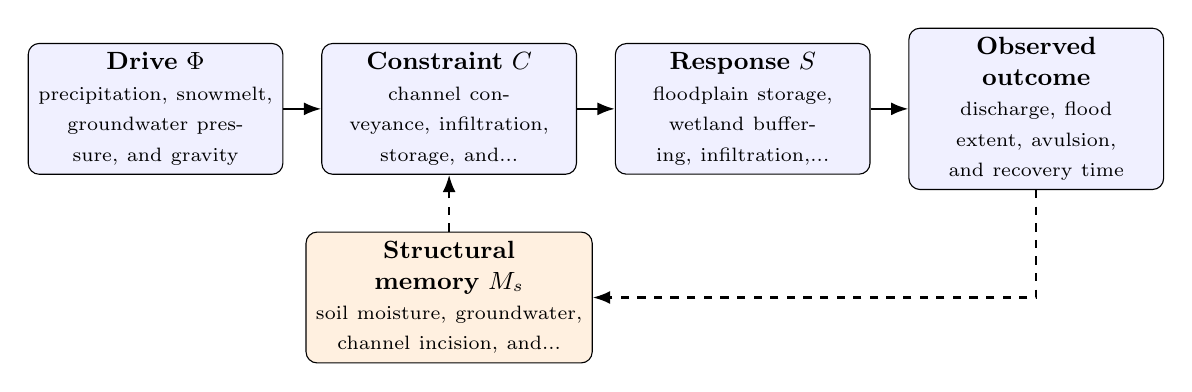
\begin{tikzpicture}[
    node distance=0.48cm,
    every node/.style={font=\small},
    box/.style={draw, rounded corners, align=center, minimum height=1.45cm, text width=3.0cm, fill=blue!6},
    memory/.style={draw, rounded corners, align=center, minimum height=1.25cm, text width=3.4cm, fill=orange!12},
    flow/.style={-{Latex[length=2.2mm]}, thick},
    feedback/.style={-{Latex[length=2.2mm]}, thick, dashed}
]
\node[box] (drive) {\textbf{Drive $\Phi$}\\\scriptsize precipitation, snowmelt, groundwater pressure, and gravity};
\node[box, right=of drive] (constraint) {\textbf{Constraint $C$}\\\scriptsize channel conveyance, infiltration, storage, and...};
\node[box, right=of constraint] (response) {\textbf{Response $S$}\\\scriptsize floodplain storage, wetland buffering, infiltration,...};
\node[box, right=of response] (outcome) {\textbf{Observed outcome}\\\scriptsize discharge, flood extent, avulsion, and recovery time};
\node[memory, below=0.72cm of constraint] (memory) {\textbf{Structural memory $M_s$}\\\scriptsize soil moisture, groundwater, channel incision, and...};
\draw[flow] (drive) -- (constraint);
\draw[flow] (constraint) -- (response);
\draw[flow] (response) -- (outcome);
\draw[feedback] (outcome.south) |- (memory.east);
\draw[feedback] (memory.north) -- (constraint.south);
\end{tikzpicture}
\caption{Paper A-04 observable CDFD/AFL architecture for Earth Hydrological Systems. Solid arrows give the proposed forward chain; dashed arrows make history-dependent feedback explicit.}
\label{fig:a04-architecture}
\end{figure}

\subsection{Paper-Specific Causal Hypothesis}

For this paper, the hypothesized causal sequence is specific. A change in
precipitation, snowmelt, groundwater pressure, and gravity arrives faster than floodplain storage, wetland buffering, infiltration, and channel adjustment can compensate.
This raises or redistributes channel conveyance, infiltration, storage, and sediment resistance. If the load persists,
the retained state encoded by soil moisture, groundwater, channel incision, and sediment legacy changes the next response, so a later event of equal
magnitude can produce a different trajectory in discharge, flood extent, avulsion, and recovery time. The
scientific task is to estimate that sequence against the best ordinary model of
the domain, not merely to redescribe the outcome after it occurs.

\subsection{Cross-Scale Translation Without Mechanistic Erasure}

For the Earth systems family, the cross-domain translation compares coupled transport, finite environmental capacity, buffering, and retained landscape or ecosystem state. It cannot erase conservation laws, geometry, or scale; it must expose where those domain equations create comparable overload and recovery structures. \cite{Holling1973,Turing1952,BakTangWiesenfeld1987}
The required scale declaration for this paper is minutes to millennia; hillslopes to continental basins. At short
scales, the key question is whether the incoming drive is transmitted,
buffered, or diverted. At intermediate scales, response changes effective
capacity and network exposure. At long scales, retained structure can alter the
state space itself. A result is genuinely cross-scale only when the aggregation
rule is stated and the same conclusion is not an artifact of averaging.

\subsection{Evidence Ladder and Discriminating Tests}

\begin{table}[htbp]
\centering
\small
\caption{Evidence ladder for Paper A-04. Each rung can fail independently.}
\begin{tabularx}{\textwidth}{|p{0.17\textwidth}|X|X|}
\hline
\textbf{Test} & \textbf{Design} & \textbf{Discriminating result} \\
\hline
Proxy audit & Measure stream gauges, soil-moisture products, topography, sediment records, and flood maps and preregister how each record maps to $\Phi$, $C$, $S$, $M_s$, and $Y$. & The mapping fails if proxies are non-identifiable, circular, or change meaning across cases. \\
\hline
Load ramp & Apply or observe an extreme rainfall pulse followed by a dry recovery interval while estimating the dominant constraint and response time. & A threshold claim requires a reproducible nonlinear change and uncertainty bounds, not a visually chosen breakpoint. \\
\hline
Recovery and memory & Match present load across units with different histories, then compare recovery paths. & The memory claim requires history-dependent divergence after current conditions are controlled. \\
\hline
Model comparison & Compare the baseline domain model with and without the CDFD/AFL state variables using held-out data. & The paper's stated falsifier is: hysteresis and recovery are explained equally well without explicit structural memory. \\
\hline
\end{tabularx}
\end{table}

\subsection{Initial One-Site Held-Out Check}

The first empirical check is deliberately narrow and reproducible. The local
analysis registration and code under
\path{Part_A_Earth_Systems/empirical_hydrology_study/} compare a native
lagged-discharge and seasonal ridge baseline with a fixed CDFD/AFL-style
extension on daily USGS Potomac River discharge (site 01646500). The
chronological 2022--2024 holdout gave an RMSE reduction of only 0.045\%, and
the 14-day moving-block bootstrap lower bound for mean squared-error reduction
was negative. Under the predeclared 1\% and positive-lower-bound rule, the
extension therefore showed no demonstrated predictive value beyond the native
baseline. This result does not test rainfall, measured channel capacity,
floodplain storage, or geomorphic memory; it prevents this paper from treating
the bookkeeping translation itself as empirical confirmation.

\subsection{Research Programme and Boundary Conditions}

The immediate research programme has four steps. First, construct a documented
dataset from stream gauges, soil-moisture products, topography, sediment records, and flood maps and retain raw units before normalization.
Second, fit a baseline domain model and report its calibration and out-of-sample
error. Third, add the smallest identifiable CDFD/AFL state extension and test
whether it improves prediction of discharge, flood extent, avulsion, and recovery time. Fourth, repeat the
analysis across the declared scale range and publish negative cases as part of
the cross-domain translation audit.

% END PART IV MAJOR CROSS-DOMAIN UPGRADE

\section{Conclusion}
Hydrology provides a direct test of flow interacting with a surface that the flow itself modifies. CDFD makes river branching comparable to other adaptive transport networks at the level of measurable topology, while the governing hydrological mechanisms remain domain specific.
\section*{Conflict of Interest} The author declares no conflict of interest.
\section*{Data Availability}
Part-specific runtime diagnostics are under each Part's \path{outputs/} directory.

Release-wide code: \path{Part_E_Synthesis/supplementary/}.

Generated summaries: \path{Part_E_Synthesis/outputs/}.

Figures: \path{Part_E_Synthesis/figures/}.


\section{Reference Layer}
\bibliographystyle{plain}
\bibliography{universal_afl_references}
\end{document}
